\section{Anhang}
\label{sec:Anhang}

\subsection{Zielsystem}
\label{sec:Zielsystem}
\begin{figure}[htb]
\centering
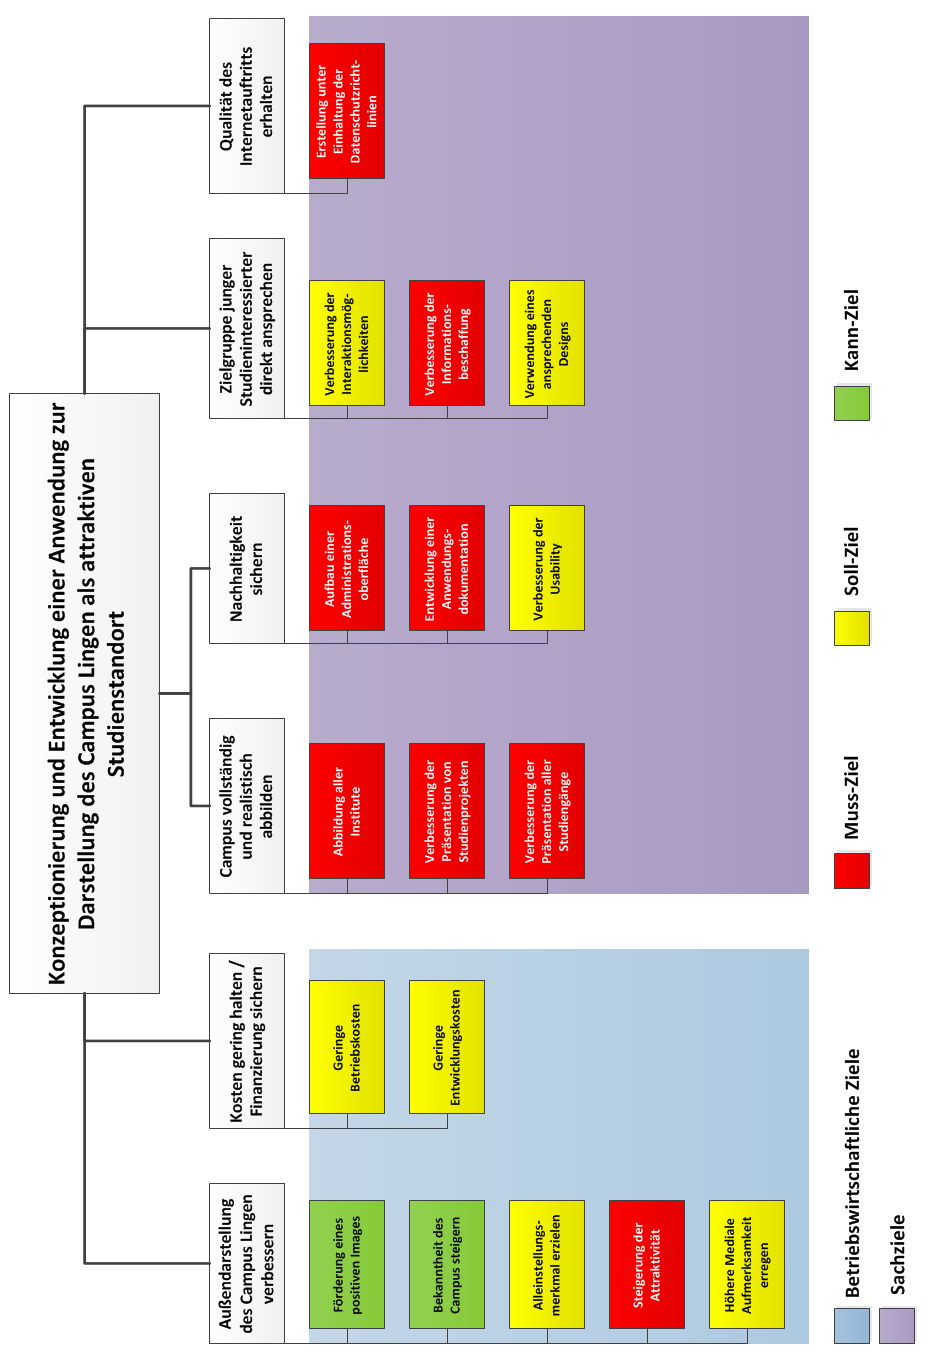
\includegraphics[height=0.7\textheight]{Zielsystem.png}
\caption[Zielsystem]{Zielsystem\protect\footnotemark}
\label{fig:Zielsystem}
\end{figure}
\footnotetext{Eigene Darstellung}

\clearpage
\begin{landscape}
  \subsection{Zielkatalog}
  \label{sec:Zielkatalog}

  \begin{figure}[htb]
    \centering
    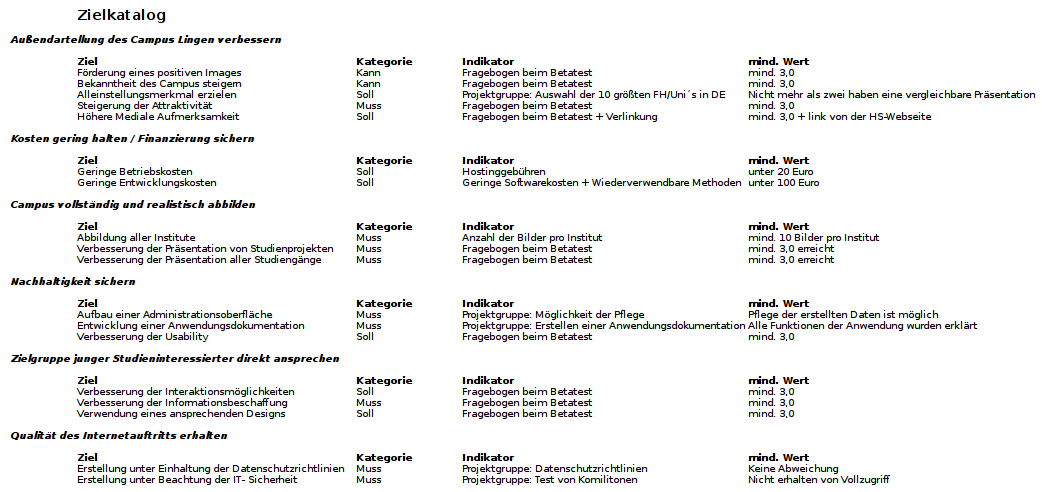
\includegraphics[height=0.7\textheight]{Zielkatalog.png}
    \caption[Zielkatallog]{Zielkatalog}
    \label{fig:Zielsystem}
  \end{figure}
\end{landscape}

\subsection{Mockup}
\label{sec:Mockup}

\begin{figure}[htb] 
\centering
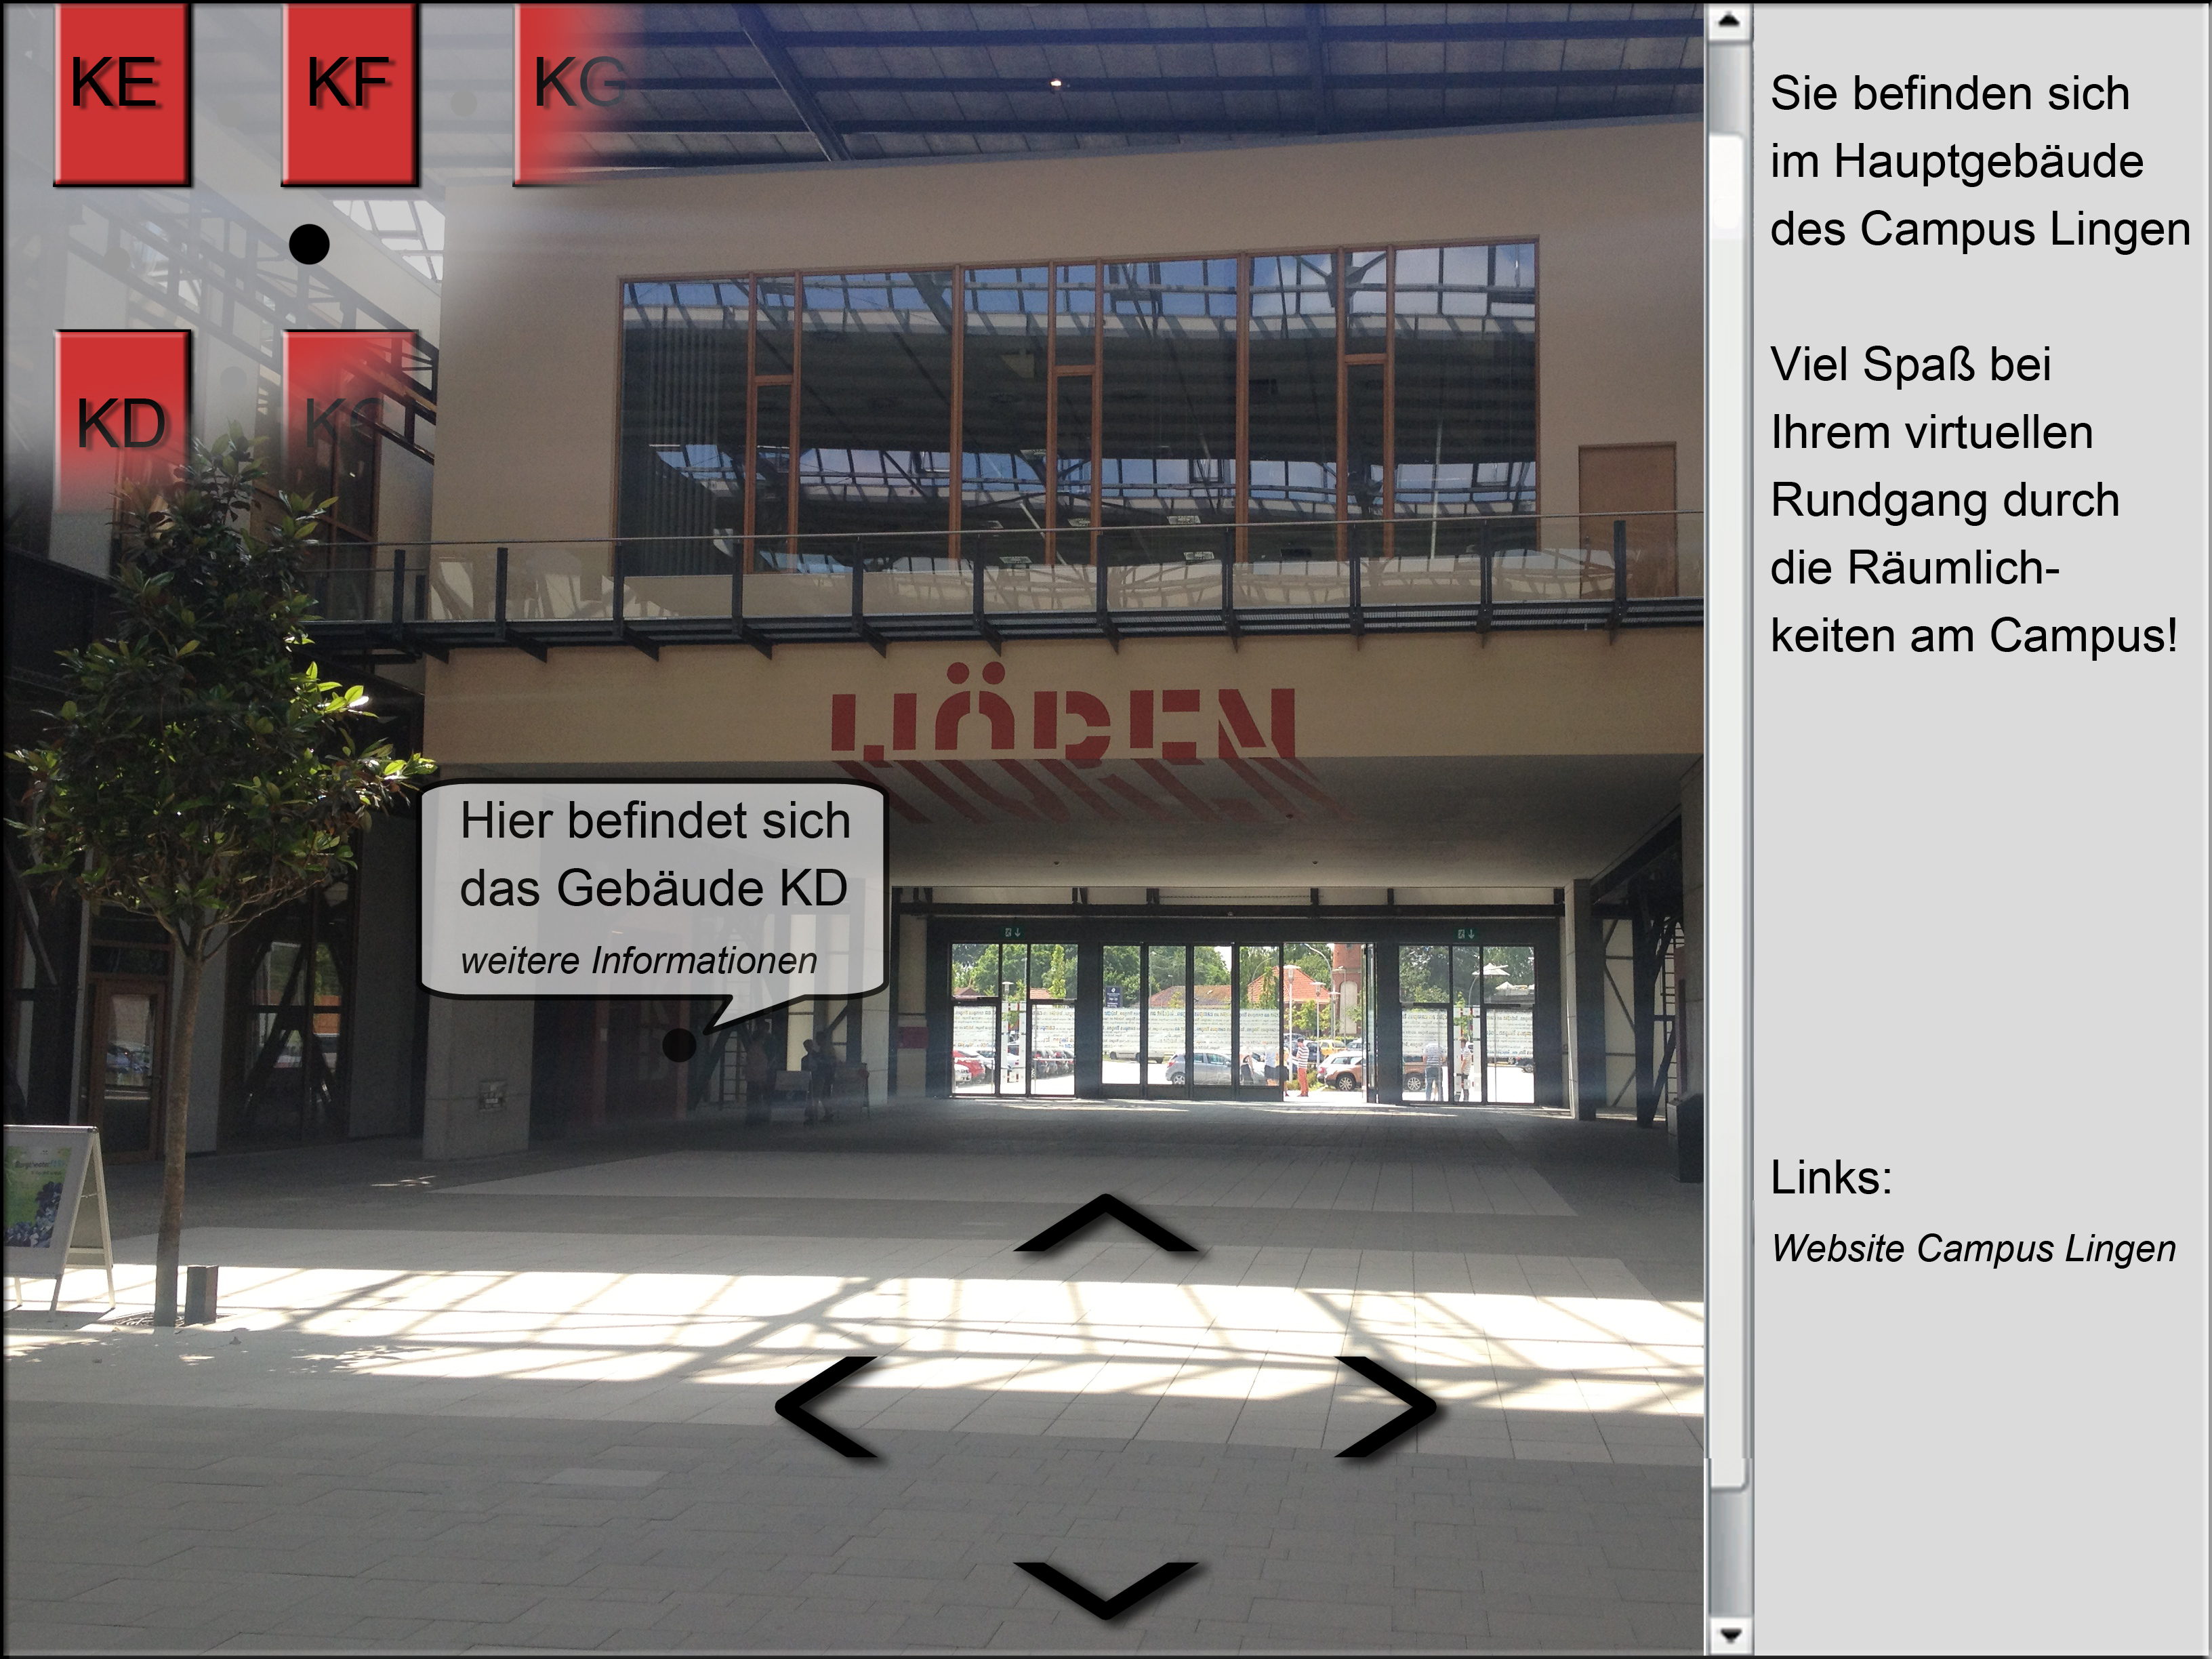
\includegraphics[width=1.0\textwidth]{MockupFrontend.jpg}
\caption[Mockup der Anwendersicht]{Mockup der Anwendersicht\protect\footnotemark}
\label{fig:MockupFrontend}
\end{figure}
\footnotetext{eigene Darstellung}

\clearpage

\begin{landscape}
  \subsection{Gantt-Diagramm}
  \label{sec:GanttDiagramm}

  \begin{figure}[htb]
    \centering
    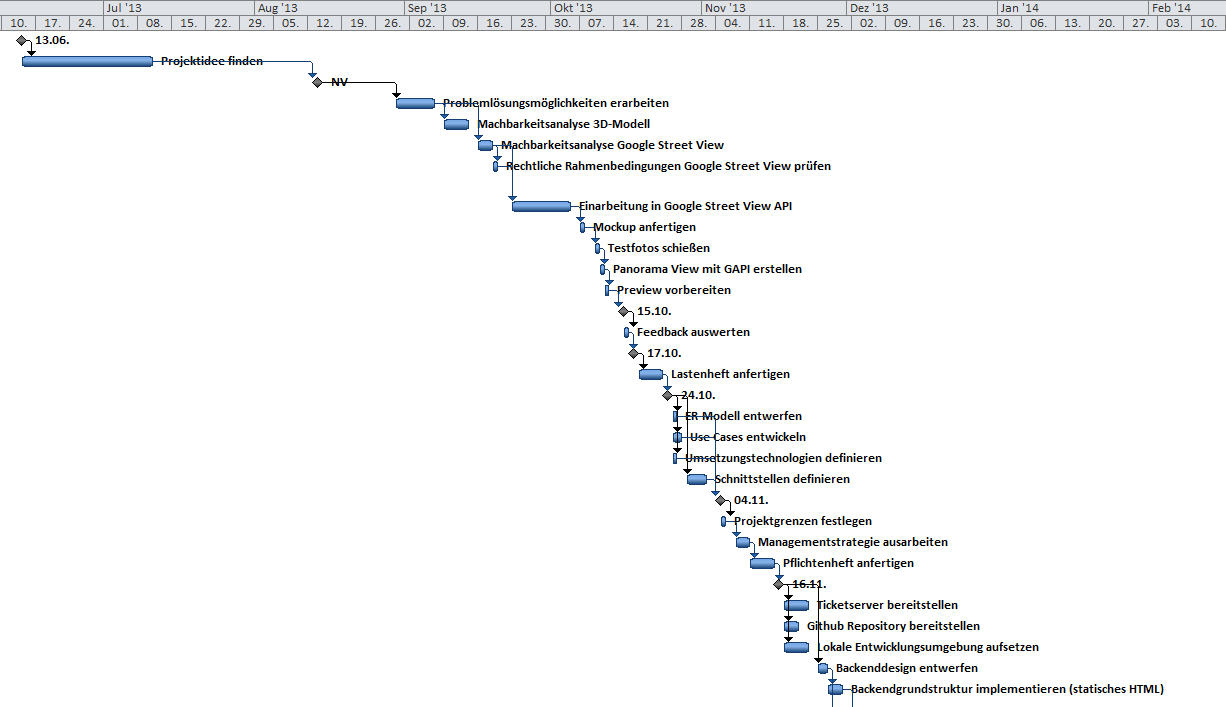
\includegraphics[height=0.7\textheight]{gantt_1.png}
    \caption[Gantt-Diagramm A]{Gant-Diagramm A}
    \label{fig:Zielsystem}
  \end{figure}

  \begin{figure}[htb]
    \centering
    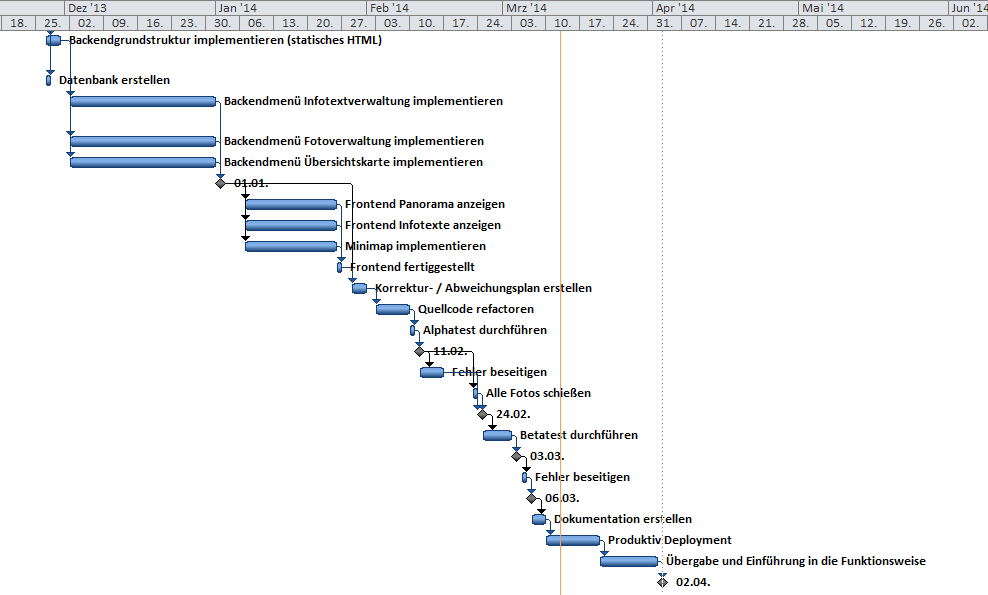
\includegraphics[height=0.7\textheight]{gantt_2.png}
    \caption[Gantt-Diagramm B]{Gant-Diagramm B}
    \label{fig:Zielsystem}
  \end{figure}
\end{landscape}


\subsection{Datenschutzrichtlinien}
\label{sec:Datenschutzrichtlinien}

Für die reibungslose Durchführung des Projektes im Bezug auf Datenschutz, ist es 
notwendig Datenschutzrichtlinien zu erstellen. Diese Richtlinien sollen dafür sorgen, 
dass die Wahrung und der Schutz von personenbezogenen Daten gewährleistet wird.

Die Datenschutzrichtlinien umfassen folgende einzuhaltende Punkte:

\begin{enumerate}
  \item Die erstellten Fotos dürfen keinen Zeitstempel (Datum, Uhrzeit) aufweisen.
  \item Es dürfen keine Personen abgebildet werden. 
  Ausnahme: Die Personen sind mit der Abbildung einverstanden und unterschreiben eine Einverständniserklärung.
  \item Es dürfen keine personenbezogenen Daten auf den Fotos erkennbar sein. Darunter fallen:
  \begin{itemize}
    \item Namen an Türschildern oder Aushängen
    \item Fotos von Personen an Aushängen, etc.
    \item Telefonnummern an Aushängen, etc.
    \item Autokennzeichen
  \end{itemize}
\end{enumerate}